\documentclass[12pt,a4paper]{article}

\usepackage[margin=1in]{geometry}
\usepackage{amsmath,amssymb,bm}
\usepackage{graphicx}
\usepackage{booktabs}
\usepackage{array}
\usepackage{float}
\usepackage{siunitx}
\usepackage{caption}
\usepackage{subcaption}
\usepackage{xcolor}
\usepackage{hyperref}
\usepackage{fancyhdr}

\hypersetup{
    colorlinks=true,
    linkcolor=blue,
    citecolor=blue,
    urlcolor=blue
}

\graphicspath{{images/}{../figures/}{./}}
\sisetup{round-mode=places, round-precision=6}

\fancyhf{}
\fancyhead[L]{CE526 Assignment 6}
\fancyhead[R]{Imran Shahriar - 2735835}
\setlength{\headheight}{15pt}
\renewcommand{\headrulewidth}{0.4pt}
\fancyfoot[C]{\thepage}
\fancypagestyle{plain}{%
    \fancyhf{}
    \fancyhead[L]{CE526 Assignment 6}
    \fancyhead[R]{Imran Shahriar - 2735835}
    \renewcommand{\headrulewidth}{0.4pt}
    \fancyfoot[C]{\thepage}
}
\pagestyle{fancy}

\begin{document}

\hypersetup{pageanchor=false}
\begin{titlepage}
    \begin{flushright}
        {\large \today\par}
    \end{flushright}

    \vspace*{0.5cm}

    \begin{center}
        
\includegraphics[width=0.42\textwidth]{metu_logo.jpg}\par
        \vspace{0.7cm}
        {\huge CE526 Assignment 6\par}
        \vspace{0.3cm}
        {\Large Finite Element Method\par}
        \vspace{0.45cm}
        {\Large Spring Semester 2025--2026\par}
        \vspace{0.45cm}
    \end{center}

    \vspace{0.9cm}

    \noindent
    \begin{minipage}[t]{0.48\textwidth}
        \raggedright
        {\Large \textbf{Submitted By}\par}
        \vspace{0.3cm}
        {\large Imran Shahriar\par}
        \vspace{0.2cm}
        {\large 2735835\par}
        \vspace{0.2cm}
        {\large MSc. in Structural Engineering\par}
    \end{minipage}
    \hfill
    \begin{minipage}[t]{0.48\textwidth}
        \raggedleft
        {\Large \textbf{Submitted To}\par}
        \vspace{0.3cm}
        {\large Prof. Ay\c{s}eg\"ul Askan G\"undo\u{g}an\par}
    \end{minipage}

    \vspace{0.5cm}

    \begin{center}
        \textbf{\large GitHub Repository:}
        \href{https://github.com/ImranMETU/CE526_Assignment6}
        {\url{https://github.com/ImranMETU/CE526_Assignment6}}
    \end{center}
    \vfill
\end{titlepage}
\hypersetup{pageanchor=true}

\section{Problem Definition}

The problem is a circular membrane of radius $R=2$ subjected to a uniformly distributed transverse load. The governing equation is
\begin{equation}
    -T\nabla^2 u = p(x,y) \qquad \text{in } \Omega,
\end{equation}
with the essential boundary condition
\begin{equation}
    u=0 \qquad \text{on } \Gamma.
\end{equation}
For this assignment,
\begin{equation}
    T=1, \qquad p(x,y)=1, \qquad R=2.
\end{equation}
Therefore, the governing equation reduces to
\begin{equation}
    -\nabla^2 u = 1.
\end{equation}

Due to the rotational symmetry of the circular domain, uniform loading, and uniform boundary condition, only one $45^\circ$ sector was modeled. The sector was discretized using one six-node quadratic triangular isoparametric element (T6) in the inner region and one nine-node biquadratic quadrilateral isoparametric element (Q9) in the outer annular region.

\section{Exact Radial Solution}

Since the exact solution is radially symmetric, the Laplacian in polar coordinates is
\begin{equation}
    \nabla^2 u = \frac{1}{r}\frac{d}{dr}\left(r\frac{du}{dr}\right).
\end{equation}
The governing equation becomes
\begin{equation}
    -\frac{1}{r}\frac{d}{dr}\left(r\frac{du}{dr}\right)=1.
\end{equation}
Multiplying by $r$ and integrating,
\begin{equation}
    \frac{d}{dr}\left(r\frac{du}{dr}\right)=-r,
\end{equation}
\begin{equation}
    r\frac{du}{dr}=-\frac{r^2}{2}+C_1.
\end{equation}
To avoid a singular derivative at $r=0$, $C_1=0$. Hence,
\begin{equation}
    \frac{du}{dr}=-\frac{r}{2}.
\end{equation}
Integrating again,
\begin{equation}
    u(r)=-\frac{r^2}{4}+C_2.
\end{equation}
Using $u(R)=u(2)=0$,
\begin{equation}
    C_2=1.
\end{equation}
Therefore, the exact solution is
\begin{equation}
    \boxed{u_{\text{exact}}(r)=1-\frac{r^2}{4}}.
\end{equation}
This exact solution is used as a numerical benchmark for the finite element solution.

\section{Finite Element Discretization}

The modeled sector is bounded by
\begin{equation}
    0 \leq r \leq 2, \qquad 0^\circ \leq \theta \leq 45^\circ.
\end{equation}
The radial interface between the T6 and Q9 elements is taken at $r=1$. The radial edges at $\theta=0^\circ$ and $\theta=45^\circ$ are symmetry boundaries. They are therefore treated as natural boundaries and are not assigned $u=0$. The essential boundary condition is applied only on the outer circular arc $r=2$.

\subsection{Global Node Table}

\begin{table}[H]
\centering
\caption{Global node coordinates and radial locations.}
\begin{tabular}{c c c c c}
\toprule
Node & Description & $x$ & $y$ & $r$ \\
\midrule
1 & Center & 0.000000 & 0.000000 & 0.0000 \\
2 & $r=1,\theta=0^\circ$ & 1.000000 & 0.000000 & 1.0000 \\
3 & $r=1,\theta=45^\circ$ & 0.707107 & 0.707107 & 1.0000 \\
4 & $r=0.5,\theta=0^\circ$ & 0.500000 & 0.000000 & 0.5000 \\
5 & $r=1,\theta=22.5^\circ$ & 0.923880 & 0.382683 & 1.0000 \\
6 & $r=0.5,\theta=45^\circ$ & 0.353553 & 0.353553 & 0.5000 \\
7 & $r=2,\theta=0^\circ$ & 2.000000 & 0.000000 & 2.0000 \\
8 & $r=2,\theta=45^\circ$ & 1.414214 & 1.414214 & 2.0000 \\
9 & $r=1.5,\theta=0^\circ$ & 1.500000 & 0.000000 & 1.5000 \\
10 & $r=2,\theta=22.5^\circ$ & 1.847759 & 0.765367 & 2.0000 \\
11 & $r=1.5,\theta=45^\circ$ & 1.060660 & 1.060660 & 1.5000 \\
12 & $r=1.5,\theta=22.5^\circ$ & 1.385819 & 0.574025 & 1.5000 \\
\bottomrule
\end{tabular}
\end{table}

The T6 element connectivity is
\begin{equation}
    \text{T6}: [1,2,3,4,5,6],
\end{equation}
and the Q9 element connectivity is
\begin{equation}
    \text{Q9}: [2,7,8,3,9,10,11,5,12].
\end{equation}
The corner nodes are ordered counterclockwise so that $\det(J)>0$ at the integration points.

\section{Weak Form and Element Matrices}

The weak form is obtained by multiplying the governing equation by a weighting function $N_i$ and integrating over the domain:
\begin{equation}
    \int_\Omega \nabla N_i \cdot \nabla u\,d\Omega = \int_\Omega N_i\,d\Omega.
\end{equation}
Using the finite element approximation
\begin{equation}
    u \approx \sum_{j=1}^{n} N_j u_j,
\end{equation}
the element equations are
\begin{equation}
    \bm{K}^e \bm{u}^e = \bm{F}^e,
\end{equation}
where
\begin{equation}
    K^e_{ij}=\int_{\Omega^e}\left(\frac{\partial N_i}{\partial x}\frac{\partial N_j}{\partial x}+\frac{\partial N_i}{\partial y}\frac{\partial N_j}{\partial y}\right)d\Omega,
\end{equation}
and
\begin{equation}
    F^e_i=\int_{\Omega^e}N_i\,d\Omega.
\end{equation}

\section{Isoparametric Mapping}

The same shape functions are used to interpolate both the geometry and the unknown field:
\begin{equation}
    x(\xi,\eta)=\sum_{i=1}^{n}N_i(\xi,\eta)x_i,
\end{equation}
\begin{equation}
    y(\xi,\eta)=\sum_{i=1}^{n}N_i(\xi,\eta)y_i,
\end{equation}
\begin{equation}
    u(\xi,\eta)=\sum_{i=1}^{n}N_i(\xi,\eta)u_i.
\end{equation}
Using the transposed Jacobian convention,
\begin{equation}
    J=\begin{bmatrix}
    x_{,\xi} & y_{,\xi}\\
    x_{,\eta} & y_{,\eta}
    \end{bmatrix}.
\end{equation}
The determinant of the Jacobian gives the local area scaling:
\begin{equation}
    d\Omega = \det(J)d\xi d\eta.
\end{equation}
The derivatives of the shape functions in global coordinates are computed from
\begin{equation}
    \begin{Bmatrix}
    N_{i,x}\\
    N_{i,y}
    \end{Bmatrix}
    =J^{-1}
    \begin{Bmatrix}
    N_{i,\xi}\\
    N_{i,\eta}
    \end{Bmatrix}.
\end{equation}

\section{Numerical Integration}

\subsection{Three-Point Quadrature for the T6 Element}

The parent triangular domain is
\begin{equation}
    0\leq \xi, \qquad 0\leq \eta, \qquad \xi+\eta\leq 1.
\end{equation}
The three-point quadrature rule used in this computation is shown in Table~\ref{tab:tri_gq}.

\begin{table}[H]
\centering
\caption{Three-point triangular quadrature rule.}
\label{tab:tri_gq}
\begin{tabular}{c c c c}
\toprule
Point & $\xi$ & $\eta$ & Weight \\
\midrule
1 & 0.0 & 0.5 & $1/6$ \\
2 & 0.5 & 0.0 & $1/6$ \\
3 & 0.5 & 0.5 & $1/6$ \\
\bottomrule
\end{tabular}
\end{table}

Therefore,
\begin{equation}
    K^e_{ij}\approx \sum_{g=1}^{3}\left(N^{(g)}_{i,x}N^{(g)}_{j,x}+N^{(g)}_{i,y}N^{(g)}_{j,y}\right)\det(J^{(g)})w_g,
\end{equation}
\begin{equation}
    F^e_i\approx \sum_{g=1}^{3}N_i^{(g)}\det(J^{(g)})w_g.
\end{equation}

\subsection{\texorpdfstring{$3\times3$}{3x3} Gauss Quadrature for the Q9 Element}

For the Q9 element, the parent domain is
\begin{equation}
    -1\leq \xi \leq 1, \qquad -1\leq \eta \leq 1.
\end{equation}
The one-dimensional Gauss points are
\begin{equation}
    \xi,\eta = -\sqrt{\frac{3}{5}},\;0,\;\sqrt{\frac{3}{5}},
\end{equation}
with weights
\begin{equation}
    w=\frac{5}{9},\;\frac{8}{9},\;\frac{5}{9}.
\end{equation}
The two-dimensional quadrature weights are products of the one-dimensional weights. Thus,
\begin{equation}
    K^e_{ij}\approx \sum_{g=1}^{3}\sum_{h=1}^{3}\left(N^{(g,h)}_{i,x}N^{(g,h)}_{j,x}+N^{(g,h)}_{i,y}N^{(g,h)}_{j,y}\right)\det(J^{(g,h)})w_gw_h,
\end{equation}
\begin{equation}
    F^e_i\approx \sum_{g=1}^{3}\sum_{h=1}^{3}N_i^{(g,h)}\det(J^{(g,h)})w_gw_h.
\end{equation}

\section{Boundary Conditions and Assembly}

After computing the T6 and Q9 element stiffness matrices and load vectors, the global system was assembled as
\begin{equation}
    \bm{K}\bm{U}=\bm{F}.
\end{equation}
There are 12 global nodes in the one-sector model. The fixed nodes are the nodes located on the outer circular boundary $r=2$:
\begin{equation}
    u_7=u_8=u_{10}=0.
\end{equation}
The free degrees of freedom are therefore
\begin{equation}
    [u_1,u_2,u_3,u_4,u_5,u_6,u_9,u_{11},u_{12}]^T.
\end{equation}
The reduced system is
\begin{equation}
    \bm{K}_{ff}\bm{U}_f=\bm{F}_f.
\end{equation}

\section{Numerical Results}

\begin{table}[H]
\centering
\caption{Finite element nodal solution and comparison with the exact radial solution.}
\label{tab:results}
\begin{tabular}{c c c c c}
\toprule
Node & $r$ & $u_{\text{FEM}}$ & $u_{\text{exact}}$ & Error \\
\midrule
1 & 0.0000 & 0.987612 & 1.000000 & -0.012388 \\
2 & 1.0000 & 0.739964 & 0.750000 & -0.010036 \\
3 & 1.0000 & 0.739964 & 0.750000 & -0.010036 \\
4 & 0.5000 & 0.943554 & 0.937500 & 0.006054 \\
5 & 1.0000 & 0.754290 & 0.750000 & 0.004290 \\
6 & 0.5000 & 0.943554 & 0.937500 & 0.006054 \\
7 & 2.0000 & 0.000000 & 0.000000 & 0.000000 \\
8 & 2.0000 & 0.000000 & 0.000000 & 0.000000 \\
9 & 1.5000 & 0.437297 & 0.437500 & -0.000203 \\
10 & 2.0000 & 0.000000 & 0.000000 & 0.000000 \\
11 & 1.5000 & 0.437297 & 0.437500 & -0.000203 \\
12 & 1.5000 & 0.437078 & 0.437500 & -0.000422 \\
\bottomrule
\end{tabular}
\end{table}

The maximum displacement occurs at the center node. The displacement decreases radially and becomes zero on the fixed circular boundary, as expected from the physical behavior of a uniformly loaded membrane.

\section{Verification Checks}

Several numerical checks were performed before accepting the solution:
\begin{enumerate}
    \item The Jacobian determinant was positive at all Gauss points.
    \item The global stiffness matrix satisfied the constant-field row-sum check before applying boundary conditions:
    \begin{equation}
        \max_i\left|\sum_j K_{ij}\right|=8.88\times10^{-16}.
    \end{equation}
    \item The total load vector before applying boundary conditions was
    \begin{equation}
        \sum_i F_i=1.569573785.
    \end{equation}
    The exact area of the $45^\circ$ sector is
    \begin{equation}
        A=\frac{1}{2}R^2\theta=\frac{1}{2}(2^2)\frac{\pi}{4}=\frac{\pi}{2}=1.570796327.
    \end{equation}
    The relative force-sum error is therefore approximately $0.078\%$.
    \item Symmetry of the solution was recovered:
    \begin{equation}
        u_2-u_3=0, \qquad u_4-u_6\approx0, \qquad u_9-u_{11}\approx0.
    \end{equation}
\end{enumerate}

\section{Radial Displacement Plot}

The assignment requires a two-dimensional radial plot rather than a three-dimensional surface plot. The radial displacement along $\theta=0^\circ$ is shown in Figure~\ref{fig:radial}. The finite element nodal values are compared with the exact solution $u(r)=1-r^2/4$.

\begin{figure}[H]
\centering
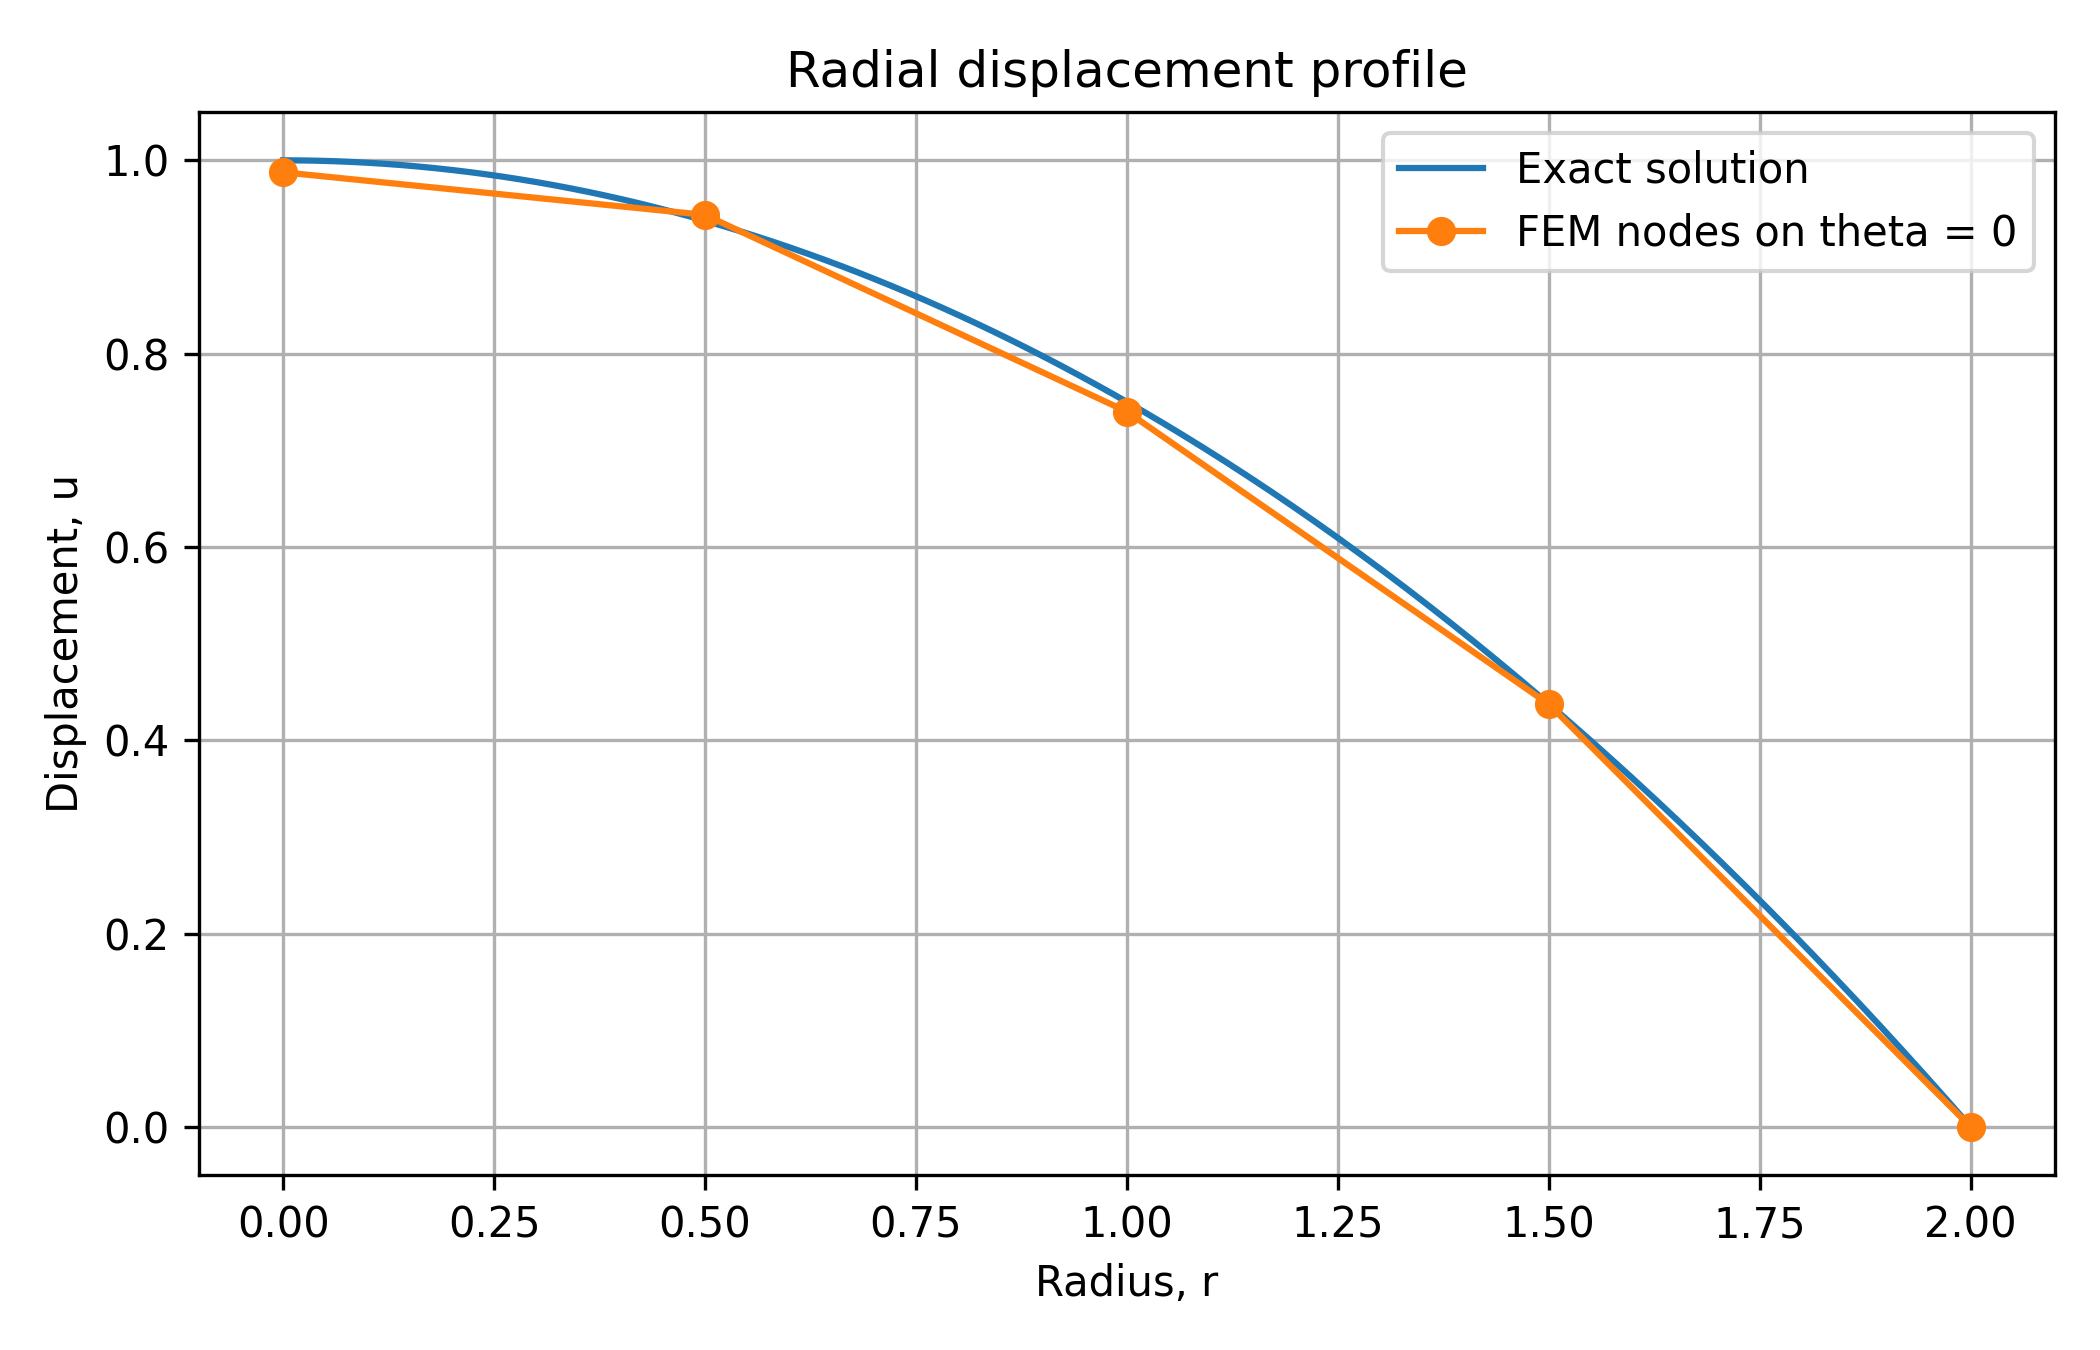
\includegraphics[width=0.85\textwidth]{ce526_assignment6_radial_2d_plot.png}
\caption{Radial displacement profile along $\theta=0^\circ$.}
\label{fig:radial}
\end{figure}

\section{Supplementary 3D Visualization}

Although the assignment asks for a two-dimensional radial plot, a three-dimensional visualization of the finite element sector solution is useful for qualitative checking. The 3D plot in Figure~\ref{fig:surface} shows the displacement field over the modeled $45^\circ$ sector.

\begin{figure}[H]
\centering
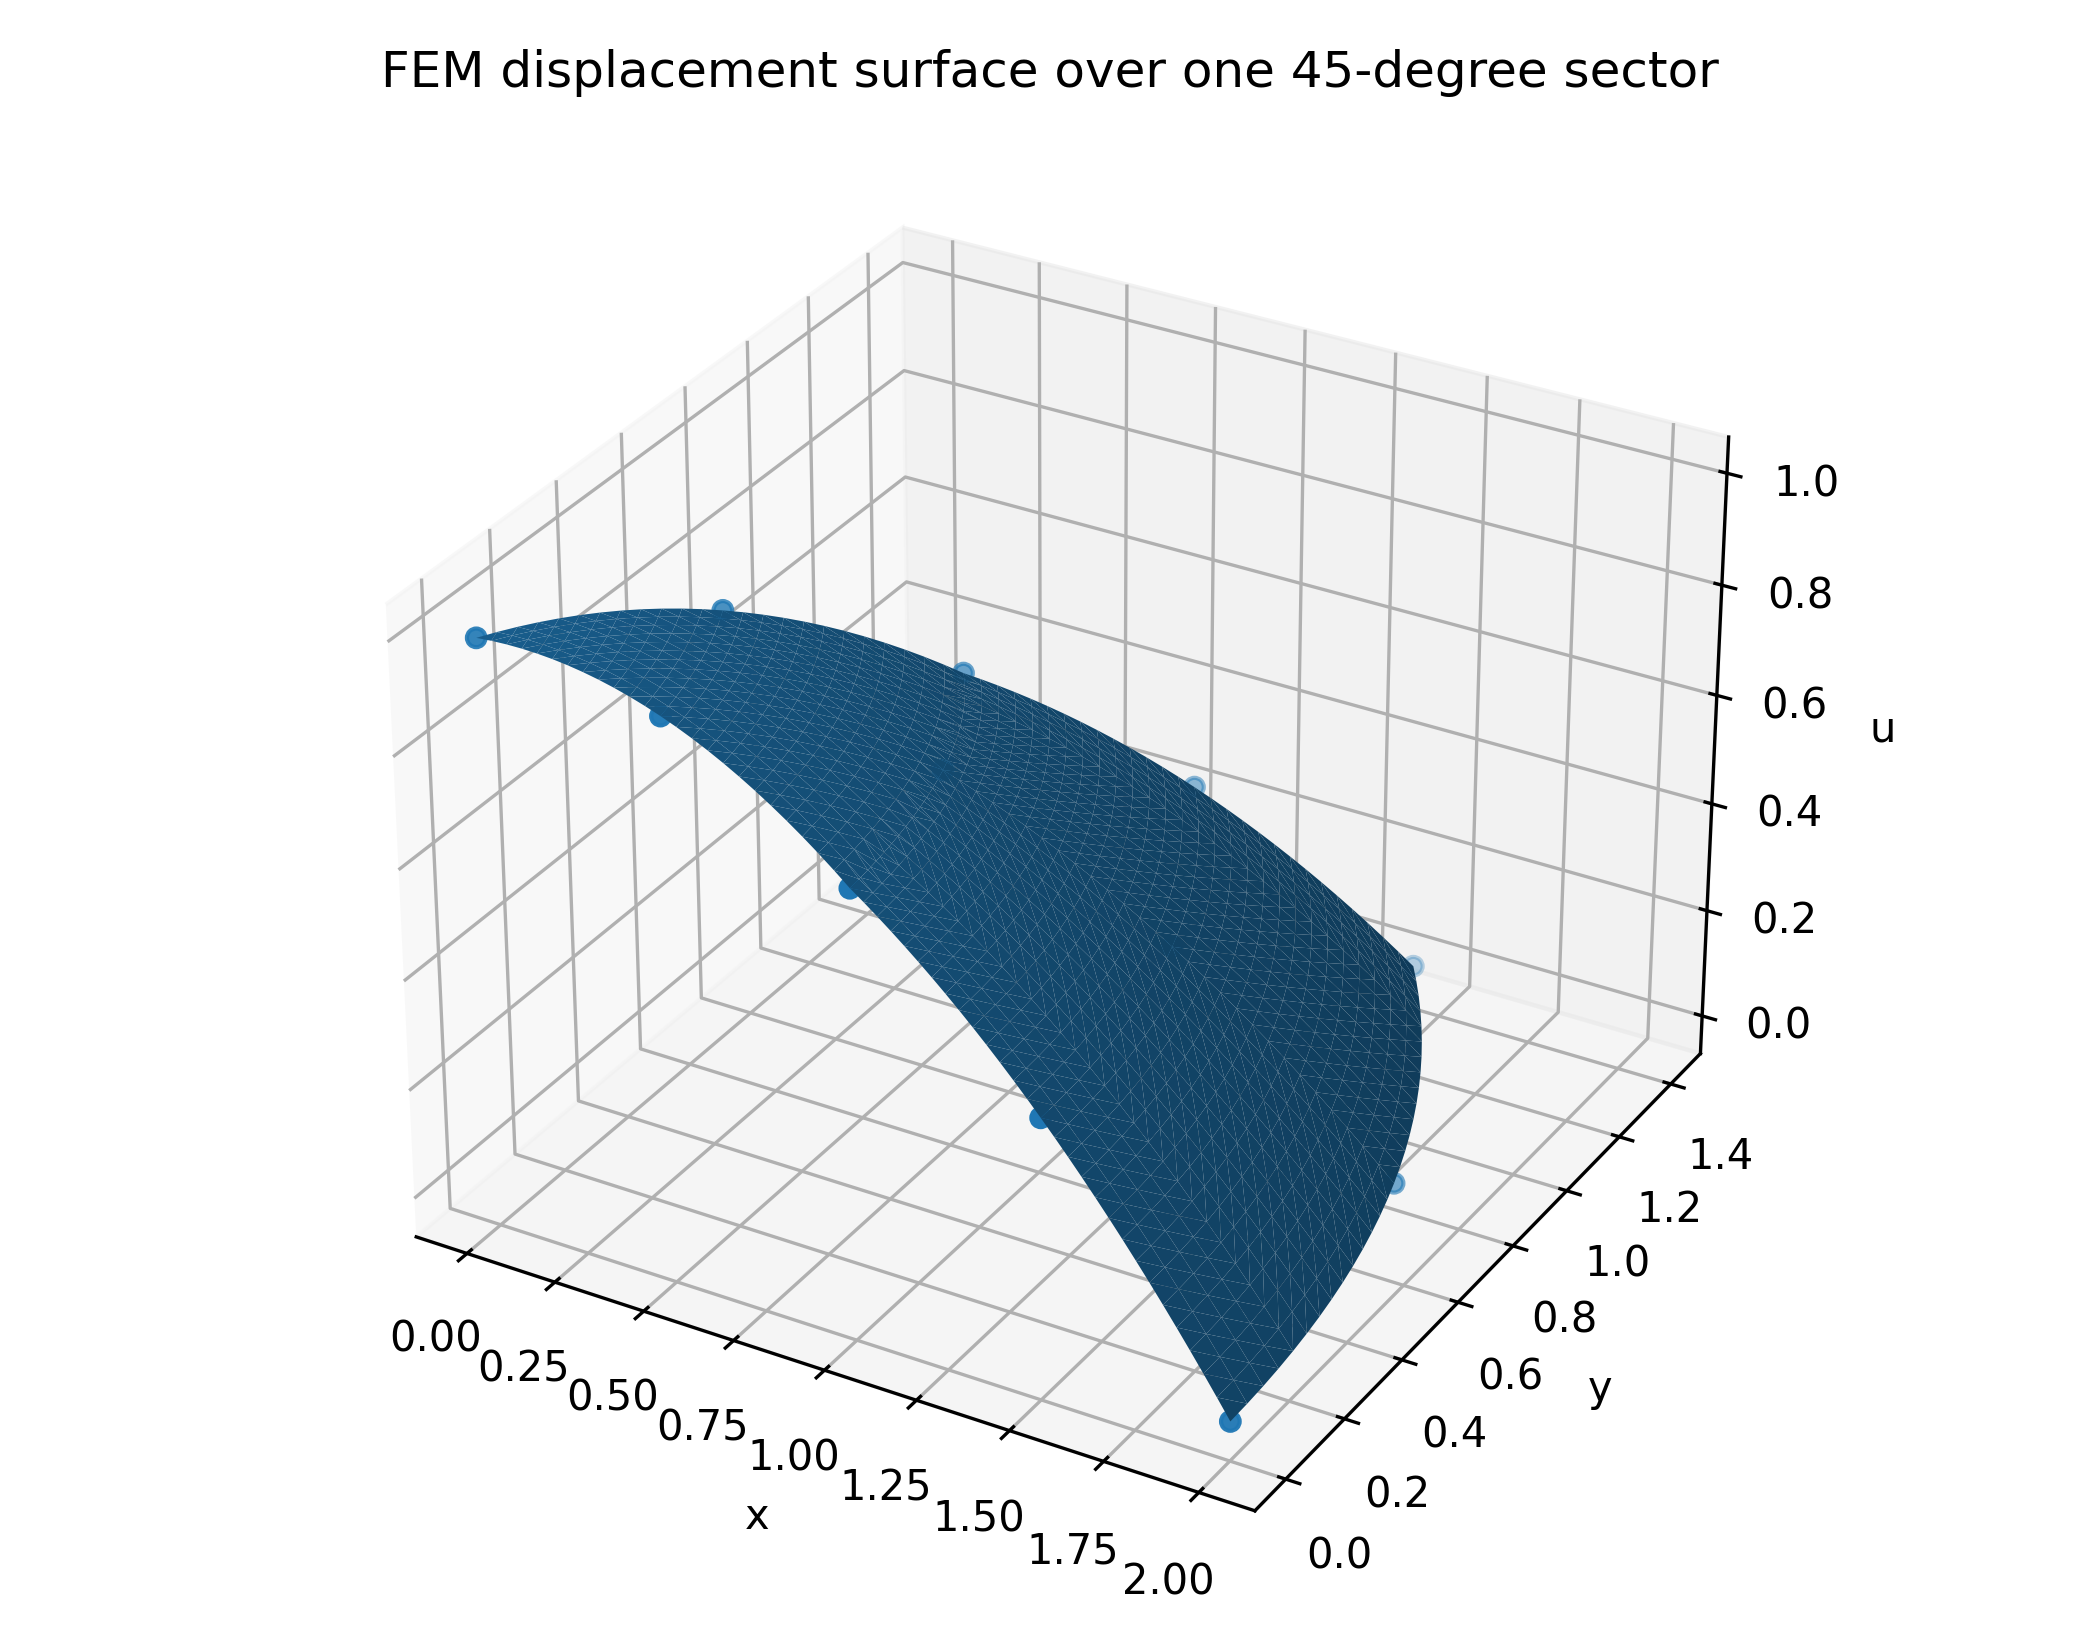
\includegraphics[width=0.85\textwidth]{ce526_assignment6_fem_sector_3d_surface.png}
\caption{Supplementary 3D visualization of the FEM solution over the modeled sector.}
\label{fig:surface}
\end{figure}

\section{Discussion}

The finite element solution is physically consistent. The largest displacement occurs at the center of the membrane and the displacement decreases toward the fixed circular boundary. The computed center displacement is $u_1=0.987612$, which is close to the exact value $u(0)=1.000000$. The largest nodal error is therefore approximately $1.24\%$ of the exact central displacement.

The agreement is particularly good in the outer Q9 element. At $r=1.5$, the computed values are approximately $0.4373$, while the exact solution is $0.4375$. The values at symmetric nodes are also identical up to numerical round-off, showing that the connectivity and boundary conditions were applied consistently.

The remaining error is mainly due to the very coarse discretization. Only one T6 element and one Q9 element were used over the sector. Although the quadratic isoparametric mapping can represent the curved boundaries more accurately than linear elements, the displacement field is still approximated by a small number of shape functions. The numerical integration rule also introduces a small approximation error, especially for curved isoparametric mappings where the Jacobian varies within the element.

The accuracy could be improved by refining the mesh in both the radial and circumferential directions, using additional sectors, increasing the number of elements through the membrane thickness direction, using higher-order elements, or using a higher-order quadrature rule such as a seven-point triangular rule for the T6 element. A convergence study comparing the numerical solution with $u_{\text{exact}}(r)=1-r^2/4$ would be the most direct way to quantify the improvement.

\section{Conclusion}

A one-sector isoparametric finite element model was used to solve the circular membrane problem. The model used one quadratic triangular element and one biquadratic quadrilateral element. The computed nodal values agree well with the exact radial solution. The maximum displacement was obtained at the center, while the displacement vanished at the outer circular boundary. The numerical checks on force sum, stiffness row sums, and symmetry confirm that the formulation and assembly are consistent.

\end{document}
